\subsection{Experiment 5: Mobile manipulators}%
\label{sub:experiment_5_mobile_manipulators}

In the final experiment, we assess the applicability of \ac{sf} and \ac{df} to a 
non-holonomic mobile manipulator. In an environment that is densely occluded by obstacles,
the motion planning problem is defined by a desired end-effector position and additional
path constraints (e.g. desired orientation of the end-effector).
\paragraph{Simulation}
In simulation, we evaluate the performance of our extension to non-holonomic
mobile manipulators with \ac{sf}. In this series, the positions of 8 obstacles
are randomized for $N=50$ cases. The workspace was limited to a
7mx7m square, so that random obstacles are ensured to be actually hindering the
motion planner. The results reveal that properties shown in the previous
experiments transfer to more complex systems without loss of the computational
benefit, \cref{fig:experiment5_simAlbert_results}. In this series, there were
1 unreached goals and 4 collisions which are, similar
to the previous experiments, caused by local minima. Local minima are more
likely for mobile manipulators as their workspace is larger.
%
\begin{figure}[h]
  \centering
  \begin{subfigure}{1.0\linewidth}
    \centering
    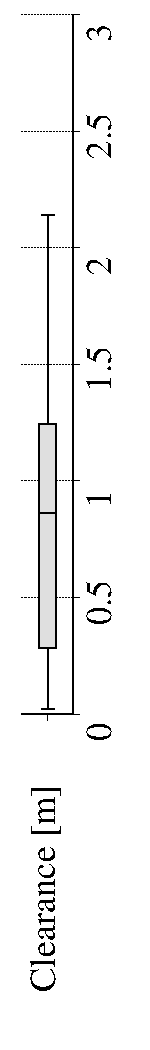
\includegraphics[angle=-90,width=\textwidth]{4_non_holonomic/simAlbert/results_fabric_clearance}
  \end{subfigure}
  \begin{subfigure}{1.0\linewidth}
    \centering
    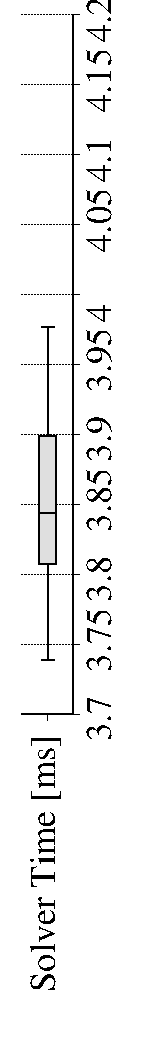
\includegraphics[angle=-90,width=\textwidth]{4_non_holonomic/simAlbert/results_fabric_solverTime}
  \end{subfigure}
  \begin{subfigure}{1.0\linewidth}
    \centering
    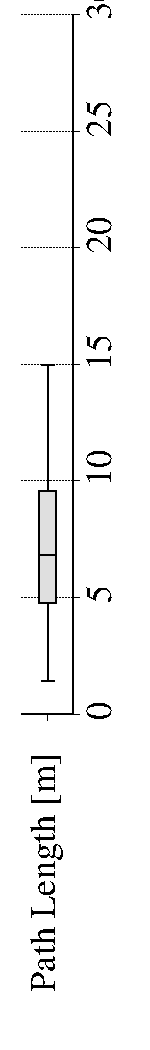
\includegraphics[angle=-90,width=\textwidth]{4_non_holonomic/simAlbert/results_fabric_pathLength}
  \end{subfigure}
  \begin{subfigure}{1.0\linewidth}
    \centering
    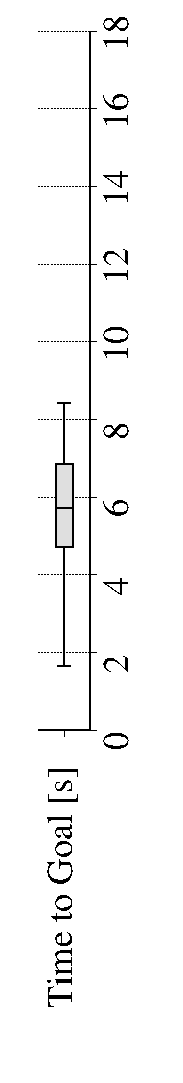
\includegraphics[angle=-90,width=\textwidth]{4_non_holonomic/simAlbert/results_fabric_time2Goal}
  \end{subfigure}
  \begin{subfigure}{1.0\linewidth}
    \centering
    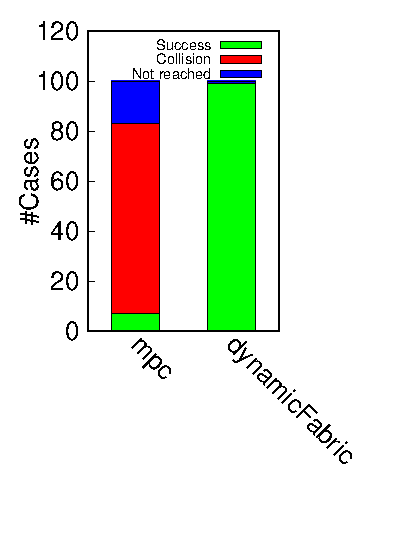
\includegraphics[angle=-90,width=\textwidth]{4_non_holonomic/simAlbert/success}
  \end{subfigure}
  \caption{Quantitative results with static fabrics for a 
    non-holonomic mobile manipulator in simulation. Fabrics solve planning problems in
    randomized environments in low planning time. This allows whole-body control and highly
    reactive behavior.
  }%
  \label{fig:experiment5_simAlbert_results}
\end{figure}
%
Combining our contributions, \ac{df} and the extension to non-holonomic robots, we
achieve reactive and safe behavior in dynamic environments. Moving obstacles are avoided in a natural way
using our method, see \cref{fig:albert_moving_obstacles}.
%
\begin{figure*}
  \centering
  \begin{subfigure}{.2\linewidth}
    \centering
    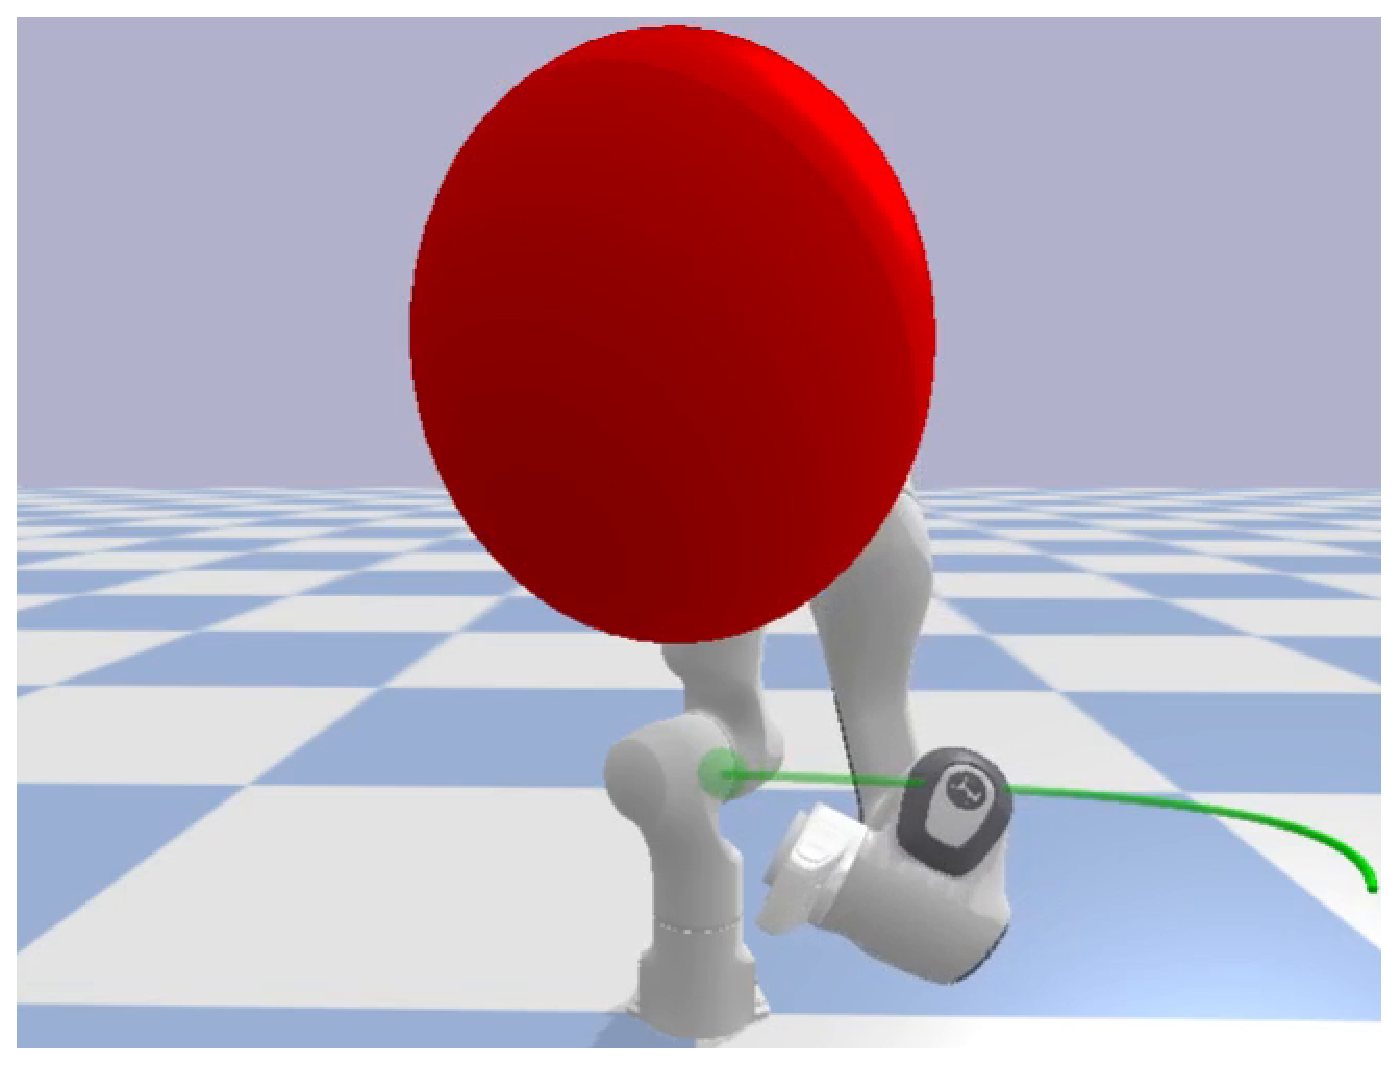
\includegraphics[width=0.9\linewidth]{4_non_holonomic/simAlbert/example_1}
  \caption{$t=0$s}
  \end{subfigure}%
  \begin{subfigure}{.2\linewidth}
    \centering
    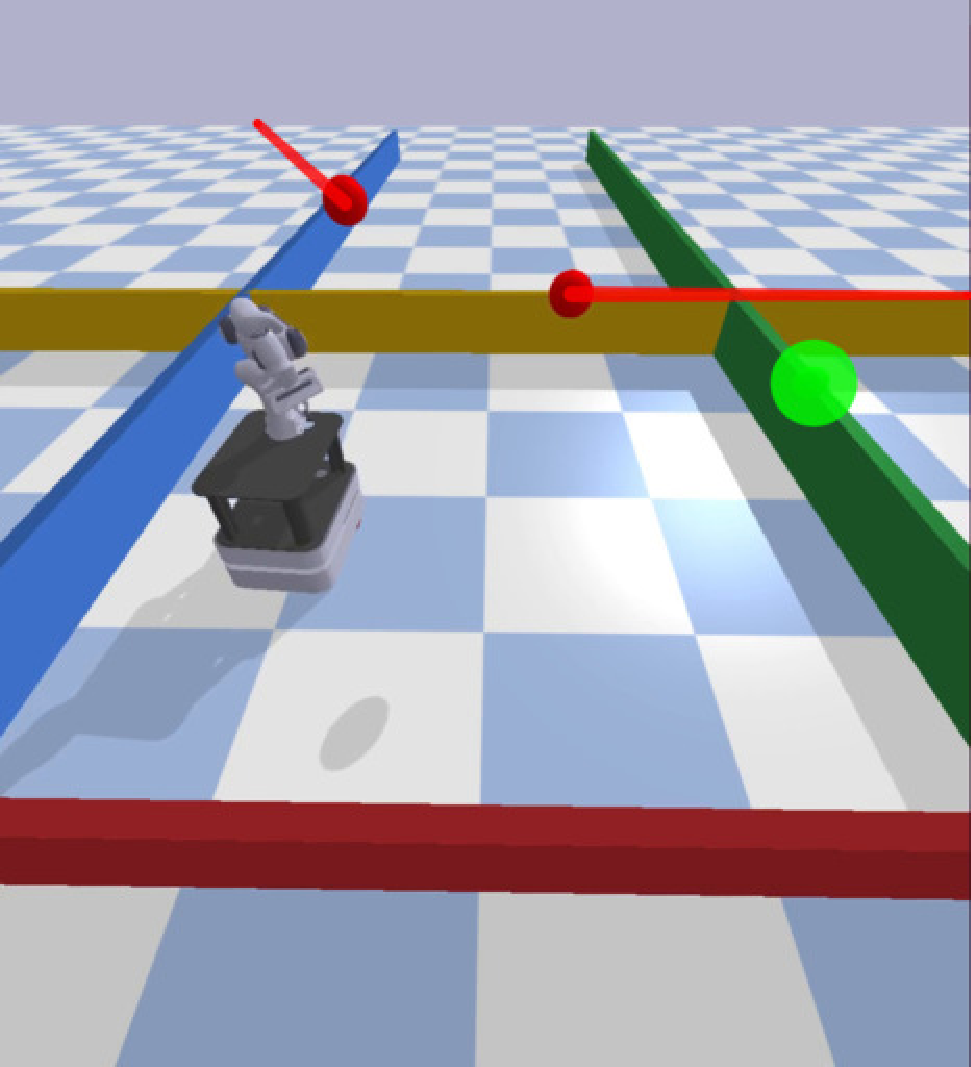
\includegraphics[width=0.9\linewidth]{4_non_holonomic/simAlbert/example_2}
  \caption{$t=7$s}
  \end{subfigure}%
  \begin{subfigure}{.2\linewidth}
    \centering
    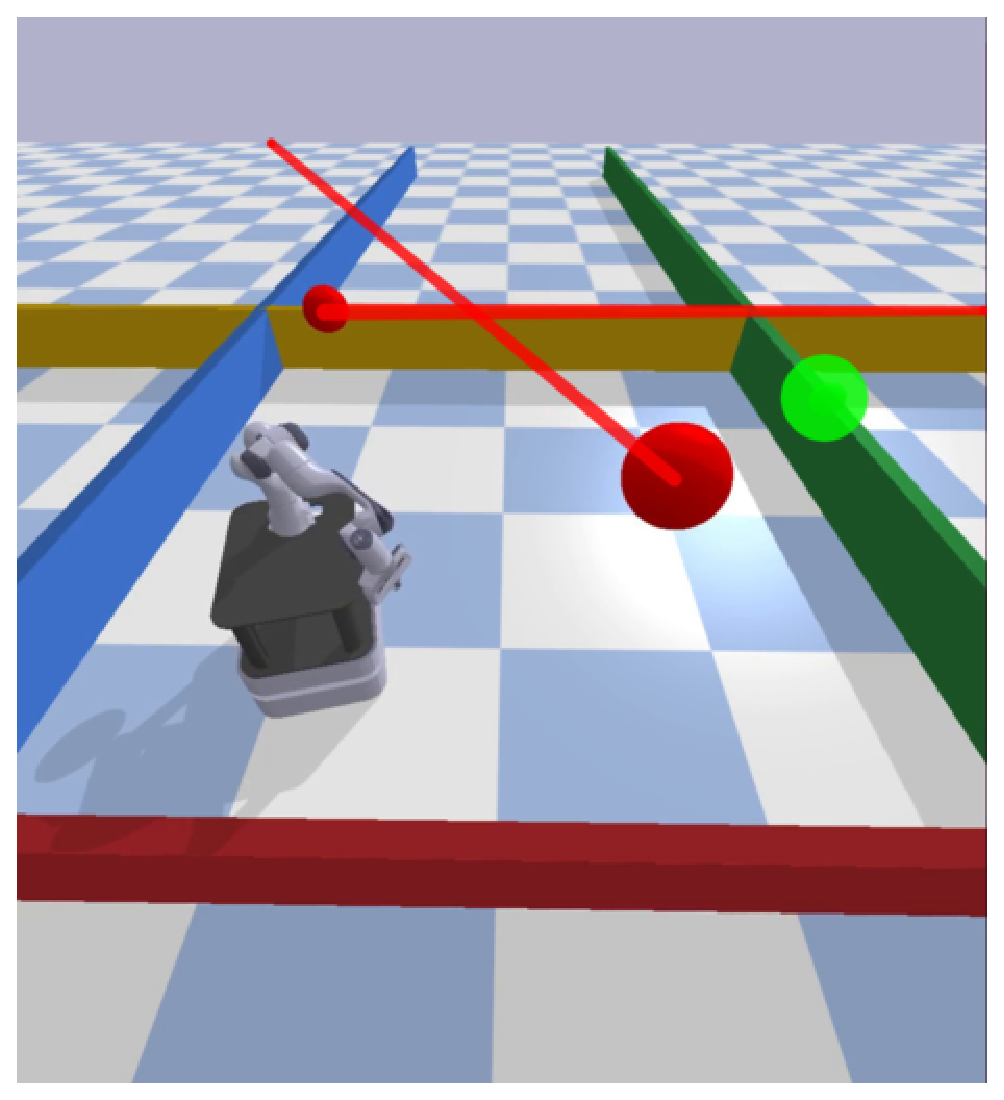
\includegraphics[width=0.9\linewidth]{4_non_holonomic/simAlbert/example_3}
  \caption{$t=14$s}
  \end{subfigure}%
  \begin{subfigure}{.2\linewidth}
    \centering
    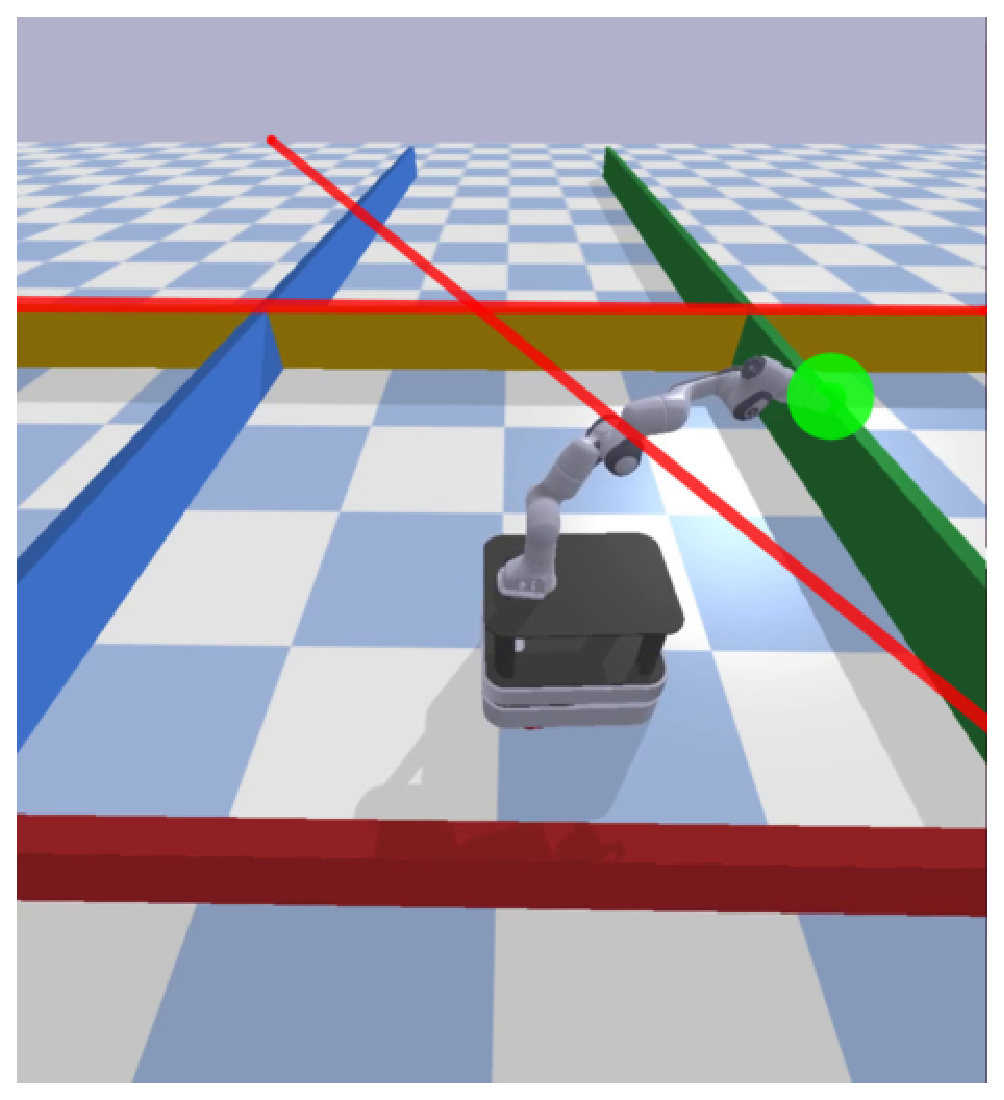
\includegraphics[width=0.9\linewidth]{4_non_holonomic/simAlbert/example_4}
  \caption{$t=20$s}
  \end{subfigure}%
  \begin{subfigure}{.2\linewidth}
    \centering
    \includegraphics[width=1.0\linewidth]{4_non_holonomic/simAlbert/trajectory}
  \caption{}%
  \label{subfig:albert_moving_obstacles}
  \end{subfigure}
  \caption{Sequence of trajectory computed with \ac{df} for a mobile manipulator in simulation with moving obstacles (red sphere with line indicating the past trajectory) and one end-effector goal (green). The trajectory of the end-effector are 
  visualized in (e) as \x{} and the desired end-effector
  position as \xt{}.
  }%
  \label{fig:albert_moving_obstacles}
\end{figure*}
%
\paragraph{Real-World}
We present qualitative results for a non-holonomic mobile manipulator using \ac{df}.
In \cref{fig:albert_spline_example}, the robot follows a trajectory defined by a basic spline,
while additionally respecting an orientation constraints on its end-effector and avoiding
the shelves and an obstacle on the ground. The end-effector trajectory is plotted in \cref{fig:albert_spline_trajectory}.
%
\begin{figure}[t!]
    \centering
    \includegraphics[width=0.9\linewidth]{4_non_holonomic/realAlbert/trajectory}
    \caption{Real-world experiment for path following with a mobile manipulator. The global path can be tracked
        accurately by \ac{df} including the extension to non-holonomic robots. The scene 
        is visualized in \cref{fig:albert_spline_example}.}
    \label{fig:albert_spline_trajectory}
\end{figure}
%
\iffalse
%
\begin{figure}[h]
  \centering
  \includegraphics[width=0.8\linewidth]{4_non_holonomic/realAlbert/motion_in_frame}
  \caption{Trajectory following with mobile manipulator. \MS{This needs to be redone \ldots}}%
  \label{fig:albert_trajectory_following}
\end{figure}
%
\fi
